\documentclass[11pt, a4paper]{jarticle}
% \documentclass{jarticle}

%% 【%】を用いた以降のその行の分を無視する
%% よって【%】はコメントアウトに使用できる

% \input{sonota/aislab_discuss} %% ディスカッション資料用の設定を読み込む
\usepackage{style/aislab}

\pagestyle{empty} %% ページ番号を消す

%% 図の挿入可
\usepackage[dvipdfmx]{graphicx} %% ←たぶんこれが一番楽
\usepackage[]{style/lastpage}
\usepackage{subcaption}

\usepackage[backend=bibtex]{biblatex}
\addbibresource{references.bib}
\defbibheading{bibliography}{\section*{参考文献}}

%%%%%%%%%%%% ページを分数形式
\makeatletter
\def\ps@myplain{\let\@mkboth\@gobbletwo%
\let\ps@jpl@in\ps@plain
\let\@oddhead\@empty
\def\@oddfoot{\reset@font\hfil- \thepage / \pageref{LastPage} -\hfil}% lastpage.tds.zipを使うことで x/最終ページ でページ数を表示できる
\let\@evenhead\@empty
\let\@evenfoot\@oddfoot}
\makeatother
\pagestyle{myplain}

% 図はfigsのサブディレクトリに集めることにする.
\graphicspath{{./figures/}}

\renewcommand{\figurename}{Fig.}
\renewcommand{\tablename}{Table}

%%%%%%%%%%%%%%%%%%%%%%%%%%%%%%%%%%%%%%%%%%%%%%%%%% ▽本文開始▽
\begin{document}


%% タイトルの設定
\jptitle{第X回:タイトル(報告書ごとに内容にふさわしいタイトルをつける) } %% 日本語タイトル
\entitle{Xth : Title (English title should be followed after Japanese title)} %% 英語タイトル
\author{M1 立命 太郎} %% 氏名
\date{2014/01/16} %% 日付

\maketitle %% タイトル作成



%%%%%%%%%%%%%%%%%%%%%%%%%%%%%%%%%%%%%%%%%%%%%%%%%%%%%%%%%%%
\noindent
$\bullet$ 前回(20xx/xx/xx)のディスカッション内容\\
ここでは前回のディスカッション内容を簡単にまとめて書く.
前回に報告した内容,議論したこと,宿題に出されたことなどを書いて
今回のディスカッションがスムーズに進行できるようにする\cite{aa}.



%%%%%%%%%%%%%%%%%%%%%%%%%%%%%%%%%%%%%%%%%%%%%%%%%%%%%%%%%%%
\section{タイトルは自由に}
章タイトルは
\verb+\section+
を使用する.必要に応じて
\verb+\subsection+
や 
\verb+\subsubsection+
を使用することによって{\bf 1.1} や {\bf 1.1.1} のように章番号を付けることができる\cite{bb}.



%%%%%%%%%%%%%%%%%%%%%%%%%%%%%%%%%%%%%%%%%%%%%%%%%%%%%%%%%%%
\subsection{文章}
文章は【です・ます】ではなく,【だ・である】にし,口語ではなく文語形式で作成する.
また,【。・、】に関しては,そのままでも良いし,【.・,】でも良い.

\section{図と表,そして式}
簡単に図,表,式等に関して説明する.ここに入れる図,表,式は必ず完成度が高いものにする.
その理由はこの資料を作成して終わりにするのではなく,
この資料を論文作成などにも利用できるようにするためである.
すなわち,一度作成したものは再利用できるように品質の高いものにする.
図や表はなるべくページの一番上か一番下に配置するのが好ましい.
\subsection{図の場合}
図を挿入する場合はキャプションを必ず書く.図番号は\LaTeX が自動で付加してくれる.
図のキャプションは図の下に書く.


\begin{figure}[b] %% h=この場所,t=ページ上,b=ページ下,p=単独ページ
	\begin{center}
	%% width は表示したい横サイズ
	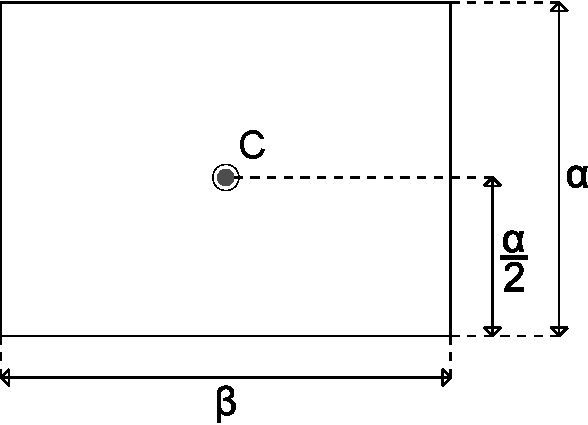
\includegraphics[width=60mm]{figure1.pdf} %% 挿入画像の指定
	\caption{図のキャプションは必ず書く} %% キャプション
	\label{figure1} %% ラベル.ラベルを書くと,\ref{}を使用して参照することができる.
	\end{center}
\end{figure}
\begin{figure}[tb] %% h=この場所,t=ページ上,b=ページ下,p=単独ページ  %% t>b の順で図の挿入場所が優先される
	\begin{center}
	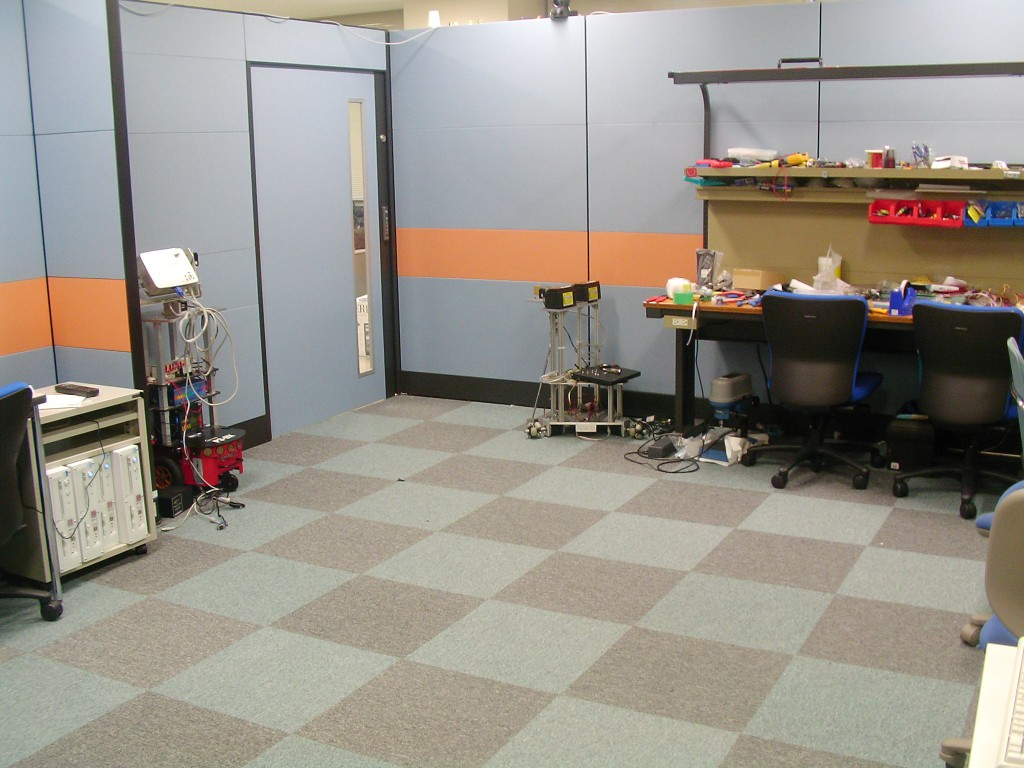
\includegraphics[width=70mm]{figure2.jpg}
	\caption{図番号は\LaTeX が自動で連番にしてくれる}
	\label{figure2}
	\end{center}
\end{figure}
ちなみに,図\ref{figure1}はベクタ形式,図\ref{figure2}はラスタ形式である.
基本的にラスタ形式(jpgやpngなど)よりもベクタ形式(epsなど)の方が,「拡大してもギザギザにならない」等の利点もあるため,読み手からは好まれる.

\pagebreak % 改ページ

\subsection{表の場合}
表も図と同様である.番号を付けた図や表は図\ref{figure1},図\ref{figure2},表\ref{table1}のように文中から参照する方が望ましい.
表のキャプションは表の上に書く.
\begin{table}[tb] %% h=この場所,t=ページ上,b=ページ下,p=単独ページ  %% t>b の順で図の挿入場所が優先される
	\caption{表の例}
	\label{table1}
	\begin{center}
	\begin{tabular}{| l | c | r |}
	\hline
	a & b & c \\ \hline
	あいう & えお & かきくけこ \\ \hline
	\end{tabular}
	\end{center}
\end{table}

\subsection{式の場合}
数式を入れるときは必ず式(\ref{equation1})のように数式番号を右に記載する.
数式番号の記載は\LaTeX が自動で行ってくれる.
\begin{equation}
\left (
\begin{array}{cc}
a & b \\
c & d \\
e & f \\
\end{array} 
\right )
\left (
\begin{array}{c}
\alpha \\
\beta \\
\end{array} 
\right )
=
\left (
\begin{array}{c}
\Phi \\
\Gamma \\
\Psi \\
\end{array} 
\right )
\label{equation1}
\end{equation}



%%%%%%%%%%%%%%%%%%%%%%%%%%%%%%%%%%%%%%%%%%%%%%%%%%%%%%%%%%%
\section{今後の計画}
最後は必ずこれからの計画を書く.やることの内容といつまで何処までをやるかを明記する\cite{cc}.
\begin{table}[h] %% h=この場所,t=ページ上,b=ページ下,p=単独ページ
	\begin{tabular}{| p{14mm} | p{90mm} |}
	\hline
	日付   & 達成内容                   \\ \hline \hline
	~x/x  & \LaTeX を勉強する          \\ \hline
	~x/xx & \LaTeX のテンプレートを作る \\ \hline
	\end{tabular}
\end{table}



%%%%%%%%%%%%%%%%%%%%%%%%%%%%%%%%%%%%%%%%%%%%%%%%%%%%%%%%%%%
% \begin{thebibliography}{9}
% \bibitem{aa} 
% あああ 参考文献は必ず文中から参照する
% \bibitem{bb}
% い 複数回参照しても構わない.
% \bibitem{cc}
% この欄の項目は,基本的には文中からの参照順に並べる
% \end{thebibliography}

\printbibliography


\end{document}